\documentclass[10pt, openany]{book}
\usepackage{header}
\pgfplotsset{compat=1.18}
\AtBeginDocument{\RenewCommandCopy\qty\SI}

\title{EE Notes}
\author{Damanic Luck}
\date{April 14, 2024}

\begin{document}
% Use this website to find symbols: https://detexify.kirelabs.org/classify.html

\maketitle
% \setcounter{chapter}{1}

\tableofcontents
\begin{todo}
    \item use this article \href{http://home.iitj.ac.in/~sptiwari/EE314/Lecture2_Semi_Basics_Junction.pdf}{to add to ch1 about doping}
    \item practice problems for ch1
    \item practice problems for ch2
    \item practice problems for ch3
    \item finish up ch3 i burned out while trying to be thorough. p117 in reader, p152 in sedra
    \item go through ch1-5 to change any units instead with the \SI{5}{\kilo \ohm} etc command OR THE \unit[per-mode=symbol]{\kilo \ohm}
\end{todo}

% CHARGE CARRIERS AND DOPING
\newpage
\section{Charge Carriers and Doping}

Doping is one method that we use in semiconductor devices

\subsection{Sources}
\begin{itemize}
    \item \href{https://www.youtube.com/watch?v=yQDfVJzEymI}{\textcolor{blue}{Razavi Electronics 1, Lec 1, Intro., Charge Carriers, Doping}}
\end{itemize}

% DRIFT AND DIFFUSION CURRENT
\newpage
\chapter{Drift and Diffusion Current}
Total current flow is made up of drift current and diffusion current. If we apply an electric field $E$ to a semiconductor crystal, then holes accelerate in the direction of $E$ and free electrons accelerate in the opposite direction of $E$. While \textbf{drift current} is movement caused by electric fields, \textbf{diffusion current} is movement caused by variation in the carrier concentration. 

\section{Drift Current}
    \[v_{p-drift} = \mu_p E, ~~~~~ v_{n-drift} = - \mu_n E\]

\begin{gline}
    \item $E$: electric field, V/cm
    \item $v_{p-drift}$: drift velocity of holes, cm/s
    \item $v_{n-drift}$: drift velocity of electrons, cm/s
    \item $\mu_p$: hole mobility, cm\sq/V $\cdot$ s, 480 cm\sq/V $\cdot$ s for intrinsic silicon
    \item $\mu_n$: electron mobility, cm\sq/V $\cdot$ s, 1350 cm\sq/V $\cdot$ s for intrinsic silicon
\end{gline}

Current density is the current per unit cross-sectional area
    \[J_p = qn\mu_p E, ~~~~~ J_n = qn\mu_n E\]
Total drift current density is
    \[J = J_p + J_n = q(p\mu_p + n\mu_n) E = \sigma E\]
Via pattern matching, we can see that conductivity $\sigma$ is given by $\sigma = q(p\mu_p + n\mu_n)$ and resistivity is the inverse of this.

\section{Diffusion Current}
\textbf{Diffusion current} is the diffusion of charge carriers that give rose to a net flow of charge fro a region of high concentration to a region of low concentration. This implies that we can have current without voltage. We can write the current density as a function of the \textbf{concentration gradient} (slope of the concentration profile) at any point such that:
    \[J_p = -q D_p \frac{dp(x)}{dx}, ~~~~~ J_n = q D_n \frac{dn(X)}{dx}\]
\begin{gline}
    \item $J_p, J_n$: hole/electron-current density, A/cm\sq
    \item $q$: magnitude of the electron charge
    \item $D_p, D_n$: diffusion constant or diffusivity of holes/electrons. For intrinsic silicon, $D_p = 12$ cm\sq/s and $D_n = 35$ cm\sq/s
    \item $p(x), n(x)$: hole/electron concentration at point $x$. Note that if $\frac{dp(x)}{dx} < 0$, $J_p$ ends up being positive.
\end{gline}
This equation shows that current density is proportional to the slope of the concentration.
The image below shows a bar of silicon and an injection of holes on the left side, which will result in hole diffusion current in the same direct (positive direction of $x$)

\begin{figure}[H]
    \centering
    \includegraphics[scale=0.5]{figs/ch02/diffusion_current.png}
\end{figure}

Suppose we fill a gas chamber that is divided into two sections with a gases of temperature $T$ on one side. If we remove this divider, the gas will fill the entire volume of the new chamber. This occurs due to the concentration gradient. If the gas molecules here were charged, there would be a net current flow.

\begin{Analysis}{Einstein Relationship}{}
    The following equation is known as the \textbf{Einstein relationship}:
        \[\frac{D_n}{\mu_n} = \frac{D_p}{\mu_p} = V_T = \frac{kT}{q}\]
    \begin{gline}
        \item $V_T$: thermal voltage; at $T \simeq 300$ K, $V_T = 25.9$ mV
    \end{gline}
    We see that the diffusion constant is related to the mobility.
\end{Analysis}
Total current will be given by the sum of drift and diffusion currents. In resistors, since the carrier is approximately uniform, diffusion current is nearly zero.
    \[J^n = J_{drift}^n + J_{diff}^n = q\mu_n n E + qD_n \frac{dn}{dx}\]

\section{Practice Problems}
\begin{enumerate}
    \item A uniform bar of $n$-type silicon of 2-$\mu$m length has a voltage of 1 V applied across it. If $N_D = 10^{16}$ \conc and $\mu_n = 1350$ cm\sq/V $\cdot$ s, find (a) the electron drift velocity, (b) the time it takes an electron to cross the 2-$\mu$m length, (c) the drift-current density, and the (d) drift current in the case that the silicon bar has a cross-sectional area of 0.25 \mun\sq.
    \begin{Ans}
        \begin{todo}
           \item TODO: finish out this question
        \end{todo}
    \end{Ans}

    \item A general relationship for the current density carried out by holes of density $p$ is $J = qpv$, where $q$ is the electronic charge and $v$ is the hole velocity.
    \begin{enumerate}
        \item Find the velocity of holes, $v(x)$, that are moving only by diffusion if they have a density distribution of $p(x) = p_0 e^{-x/l}$ . The electric field is zero.
        \item What would be the electric field that would lead to a hole drift velocity equal to that of the diffusion velocity in part(a)? Use Einstein's relation to answer this question.
        \item At 300 K, what is the value of $l$ to make the ecltric field in part (b) be 1000 V/cm?
    \end{enumerate}
\end{enumerate}

\section{Sources}
\begin{itemize}
    % \item \href{https://www.youtube.com/watch?v=NWolpDgi6_Y}{\textcolor{blue}{Razavi Electronics 1, Lec 2. Doping, Drift}}
    \item Sedra, Adel S., et al. Microelectronic Circuits. Oxford University Press, 2021
    \item \href{https://file.notion.so/f/f/048d6522-202b-48d4-b5d9-bc005bd602e2/214bf1f0-292f-48d6-9016-737d9f5da155/ee105_reader_v3.pdf?id=237a4300-3dbe-47d1-888b-ffae90d8352b&table=block&spaceId=048d6522-202b-48d4-b5d9-bc005bd602e2&expirationTimestamp=1714435200000&signature=yx-H1qvZJIodPfazOpwXX0Ce2mWMG8skOHl45xoPxus&downloadName=ee105_reader_v3.pdf}{EE105 Reader}
    \item Q2 fro here is Q2 from EE105 HW6
\end{itemize}

% PN JUNCTIONS
\newpage
\section{PN Junctions}

A \textbf{PN junction} is the junction between an $N$-type semiconductor and $P$-type semiconductor. Understanding the PN junction will set up us for understanding diodes, BJTs, and MOSFETs later. It seems like we draw it as two separate silicon crystals, but in actual practice the $p$ and $n$ regions are part of the same silicon crystal, accomplished by creating regions of different doping.

Plus ("+") signs represent majority holes while minus ("-") signs represent majority el ectrons. The following diagram is from Seda and Adel's \textit{Microelectronic Circuits}.

\begin{figure}[H]
    \centering
    \includegraphics[scale=0.5]{figs/ch03/pn_junction.png}
    \caption{Simplified physical structure of the PN junction}
\end{figure}

\subsection{Diffusion Current}
Although it doesn't show it in the diagram, there minority holes generated by thermal ionization in the $n$-type material and there are minority electrons generated in the $p$-type material. Due to concentration difference of holes in the $p$ region and the $n$ region, holes diffuse across the junction from the $p$ side to the $n$ side. This results in \textbf{diffusion current, $I_D$}, whose direction is from the $p$ to $n$ side.

So current Damanic is wondering right now "if this stuff is diffusing then won't this entire block be the same mush at the end." Here we introduce the depletion region. Holes that diffuse across the junction into the $n$ region recombine with majority electrons there. A charge is said to be \textbf{uncovered} when some of the bound positive charge is no longer neutralized by free electrons. This introduces the idea that at a region close to the junction, it is depleted of free electrons and contains unbound positive charge for the $n$ region.

\begin{figure}[H]
    \centering
    \includegraphics[scale=0.5]{figs/ch03/uncovered_region.png}
    \caption{Top image shows PN-junction with bound charges and bottom image is potential along an axis perpendicular to the junction}
    \label{fig:barrier-voltage1}
\end{figure}

The left side of the PN junction ($p$ region) will be negatively charged while the right side ($n$ region) will be positively charged. To sum it up, this is because at some point, electrons that diffuse across the junction into the $p$ region will recombine with holes, and those holes will disappear leaving uncovered bound negative charge. Vice versa for holes diffusing into the $n$ region. 

From the figure above we see that the $n$ region will be positively charged and the $p$ side if negatively charged. This is the \textbf{depletion region}, or the \textbf{space-charge region} or \textbf{depletion layer}. There are no \textit{mobile} charge carriers present here. Charges on both sides of the depletion region results in an electric field $E$. Here we introduce the idea that a larger barrier voltage results in a small number of carriers that can overcome this barrier. This leads to a decrease in magnitude of diffusion current since it is more difficult for holes to diffuse into the $n$ region and electrons to diffuse into the $p$ region. Referring again to figure \ref{fig:barrier-voltage1}, we see that $V_0$ is the barrier voltage. Therefore the diffusion current $I_D$ has a strong relationship with $V_0$, the voltage drop across the depletion region.

\subsection{Drift Current and Equilibrium}
Recall that drift current is caused by electric fields and $I_S$ is independent of the value of the depletion-layer voltage $V_0$. Under open-circuit conditions, there is no external current, so 
    \[I_D = I_S\]
This condition is maintained by $V_0$.
\begin{Analysis}{$I_S$ and $I_D$ at Equilibrium}{}
    \begin{gline}
        \item $V_O$: barrier voltage
        \item $I_S$: drift current whose direction is from the $n$ side to the $p$ side of the junction
        \item $I_D$: diffusion current whose direction is from the $p$ side to the $n$ side of the junction
    \end{gline}
    \begin{enumerate}
        \item \textbf{$I_D > I_S$}: more bound charge is uncovered on both sides $\rightarrow$ the depletion layer widens (vertically)$\rightarrow$ $V_0$ increases $\rightarrow$ $I_D$ decreases until $I_D = I_S$ (equilibrium)
        \item \textbf{$I_D < I_S$}: uncovered charge decreases $\rightarrow$ depletion layer narrows (vertically) $\rightarrow$ $V_0$ decreases $\rightarrow$ $I_D$ increases until $I_D = I_S$ (equilibrium)
    \end{enumerate}
\end{Analysis}

Under the zero bias equilibrium condition (no external voltage is applied to the PN junction), does the diffusion and drift current "cancel" out here, meaning that current density is zero. Their individual components are also equal here, i.e. hole/electron drift current is equal to hole/electron diffusion current, respectively.
    \[J_n = 0 = qn_0 \mu_n E_0 + q D_n \frac{dn_0}{dx}\]

$V_0$ has been referred to so far as barrier voltage boltage, but it's also called \textbf{junction built-in voltage}.
    \[\phi_{bi} = V_{th} \ln \left(\frac{N_A N_D}{n_i^2}\right) = \frac{kT}{q} \ln \left(\frac{N_A N_D}{n_i^2}\right)\]
Remember here that $V_th$ is thermal voltage which is $\approx$ 26 mV at room temperature. $\phi_{bi}$ is typically 0.6 V to 0.9V for room temperature silicon. In the EE105 reader, $\phi_{bi}$ and $V_{th}$ has the same meaning as $V_0$ and $V_T$, respectively, in the \textit{Microelectronic Circuits} textbook. I'm writing down the EE105 reader notation here for clarity.

\begin{figure}[H]
    \centering
    \includegraphics[scale=0.6]{figs/ch03/3_graph.png}
    \caption{Graphs of (a) a PN junction (b) carrier concentrations (c) charge density (d) built in voltage $V_0$}
    \label{fig:3figs}
\end{figure}
How we got from each graph.
\begin{itemize}
    \item 
\end{itemize}

\begin{figure}[H]
    \centering
    \includegraphics[scale=0.5]{figs/ch03/concentration_reader.png}
    \caption{Graph of electric field of PN junction}
    \label{fig:electric_fields_pn}
\end{figure}
Here in figure \ref{fig:electric_fields_pn}, the electric fields in the depletion region are negative because positive charges are on the right and the negative charges are on the left, assuming zero fields in neutral $P$-region and $N$-regions. Key takeaways:
\begin{pline}
    \item Width of the depletion region is not symmetric
    \item The negative peak of the electric field always occurs at the junction
\end{pline}

\subsection{Reverse Bias}

\subsection{Forward Bias}

\subsection{PN Junction with External Voltage Applied}
The above section was discussing the PN junction at equilibrium.

\subsection{Practice Problems}
\begin{enumerate}
    \item Show that 
        \[V_0 = \frac12 (\frac{q}{\epsilon_s})(\frac{N_A N_D}{N_A + N_D}) W^2\]
    % \begin{Ans}
    %     We know that $\phi_{bi} = V_{th} \ln \left(\frac{N_A N_D}{n_i^2}\right) = \frac{kT}{q} \ln \left(\frac{N_A N_D}{n_i^2}\right)$
    % \end{Ans}
    \item Show that for a PN junction in which the $p$ side is much more heavily dped than the $n$ side (i.e. $N_A \gg N_D$) referred to as a $p^+ n$ diode. The following can be written as follows:
        \begin{align*}
            W &\simeq \sqrt{\frac{2 \epsilon_s}{q N_D}V_0}, ~~~~~ x_n \simeq W, ~~~~~ x_p \simeq \frac{W}{N_A / N_D} \\
            Q_j &\simeq A q N_D W, ~~~~~ Q_j \simeq A \sqrt{2 \epsilon_s q N_D V_0}
        \end{align*}
    
    \item 
\end{enumerate}

\subsection{Sources}
\begin{itemize}
    \item Sedra, Adel S., et al. Microelectronic Circuits. Oxford University Press, 2021: Specifically screenshots of the graphs I need to redo this when I learn how to use graphing/tikzpicture better in LaTex
    \item \href{https://file.notion.so/f/f/048d6522-202b-48d4-b5d9-bc005bd602e2/214bf1f0-292f-48d6-9016-737d9f5da155/ee105_reader_v3.pdf?id=237a4300-3dbe-47d1-888b-ffae90d8352b&table=block&spaceId=048d6522-202b-48d4-b5d9-bc005bd602e2&expirationTimestamp=1714435200000&signature=yx-H1qvZJIodPfazOpwXX0Ce2mWMG8skOHl45xoPxus&downloadName=ee105_reader_v3.pdf}{EE105 Reader}
\end{itemize}

% MOSCAP
\newpage
\chapter{MOS Capacitor}
The MOS in MOS capacitor stands for Metal-Oxide-Silicon. Sometimes the S is also written as substrate in other places. Understanding threshold voltage here for a MOS-CAP is useful for also understanding MOSFETs in a later chapter.
\begin{pline}
    \item Metal: usually this ia  heavily doped polysilicon (Poly-$Si$) layer doped with $n^+$ or $p^+$, due to high temperature processing for aluminum
    \item Oxide: SiO$_2$ where $\epsilon_{ox} = 3.9 \epsilon_0$, can be any insulator actually
    \item Substrate: $\epsilon_s = 11.7 \epsilon_0$; NMOS capacitor $\rightarrow$ $P$-type substrate, PMOS capacitor $\rightarrow$ $N$-type substrate
\end{pline}

\section{MOSCAP at Equilibrium}
\begin{figure}[H]
    \centering
    \includegraphics[scale=0.4]{figs/ch04/moscap_short.png}
    \caption{MOS CAP with gate and body shorted in equilibrium}
    \label{fig:moscap_short}
\end{figure}
In equilibrium , the gate and body, which are the terminals where voltage is applied, are shorted like in fig \ref{fig:moscap_short}. Under thermal equilibrium, there is no current flow, so an $N$ type polysilicon gate will rise to a higher potential than the $P$ type substrate like in a PN junction (previous chapter is relevant here). We also assume that the material used to short the body and the gate is made of the gate material, so it looks more like this.
\begin{figure}[H]
    \centering
    \includegraphics[scale=0.4]{figs/ch04/moscap_short2.png}
    \caption{There is a $\phi_{bi}$ from across the PN junction that leads to potential drop across the oxide}
\end{figure}

\begin{gline}
    \item[] Potential of the $P$ type region substrate: $\phi_p = -(\frac{kT}{q}) \ln(\frac{N_A}{n_i})$ 
    \item[] Potential of the $N$ type gate: $\phi_{poly,n+} = (\frac{kT}{q}) \ln(\frac{N_{d,poly}}{n_i})$
    \item[] Built in potential, NMOS Cap: $\phi_{bi} = \phi_{poly,n+} - \phi_p$
\end{gline}
In practice, real wires made of metal like aluminum or copper are used to connect the gate to the body. At the body side, this metal is connected to a heavily doped $p^+$ region. The \textbf{flatband voltage}, $V_{FB}$, is defined as the gate to body voltage that results in net zero charge and zero fields in the MOSCAP structure. The name comes from the observation that energy bands are flat whe the charge on the gate goes to zero and the depletion region disappears.
    \[V_{FB} = -\phi_{bi} = -(\phi_{n^+} - \phi_p)\]

Due to the difference in materials that make up the gate and body, we have an electric field from the gate to the body. 
\section{Regions of Operation}
There are three regions of operation: accumulation, depletion, and inversion. 

\subsection{Accumulation}
The MOSCAP operates under accumulation when $V_{GB} < V_{FB}$. $V_{GB}$ is the gate to body voltage. This looks like a parallel plate capacitor where there are many electrons and holes to charge up the plates. Negative charges/electrons can flow into the gate and holes will \textbf{accumulate} on the surface of the device. This is because negative bias attracts holes to reside under the gate. 

\subsection{Depletion}
The MOSCAP operates under depletion when $V_{GB} > V_{FB}$. An artificial depletion region is formed if you apply a voltage to the gate of the MOS CAP. When this happens we are in depletion mode. This is similar to the MOS CAP being in equilibrium.

\subsection{Inversion}
The MOSCAP operates under inversion when $V_{GB} = V_{FB}$.
\begin{todo}
    \item might be a good idea to expand on this
\end{todo}

\section{Practice Problems}

\begin{enumerate}
    \item For a MOSCAP with a $p$-type substrate. Given $V_{FB} = -0.53$ V, $N_A = 10^{17}$\conc, oxide (SiO$_2$ $\epsilon_{ox} = 4\epsilon_0$) thickness of 3nm, and Silicon $\epsilon_{Si} = 12\epsilon_0$. At 300K and $n_i = 10^{10}$\conc. The right-hand side is the semiconductor.
    \begin{enumerate}
        \item What is the condition for inversion to happen? Do not just answer $V > V_T$.
        \begin{Ans}
            For inversion to happen, the gate-base voltage is greater than the threshold voltage of the MOSCAP $V_{GB} > V_T$. This happens because the depletion region stops growing as the gate voltage is increased due to surface potential increasing. Surface potential will increase until the electron density at the surface equals the background ion density. This then leads to the surface effectively becoming an $N$-type.
        \end{Ans}

        \item Qualitatively draw the charge, electric field, and potential at accumulation.
        \item Qualitatively draw the charge, electric field, and potential at depletion.
        \item Qualitatively draw the charge, electric field, and potential at inversion.
        \item Calculate the surface potential at the threshold. Hint: {\large $n = \frac{n_i^2}{N_A} e^{\frac{q\phi_s}{kT}}$}
        \begin{Ans}
            We see here that surface potential is half of the body potential.
            \begin{align*}
                \phi_S &= 2\phi_B \\
                &= 2(\frac{kT}{q}) \ln(\frac{N_A}{n_i}) \\
                &= 2(0.026 \mathrm{V}) \ln(\frac{10^{17} \mathrm{cm}^{-3}}{10^{10} \mathrm{cm}^{-3}}) \\
                &= 0.838 \mathrm{V}
            \end{align*}
        \end{Ans}

        \item Calculate the depletion width and depletion charge density at the threshold. Hint: {\large $W_D = \sqrt{\frac{2 \epsilon_{Si} \phi_s}{q N_A}}$}
        \begin{Ans}
            \begin{align*}
                W_D
            \end{align*}
        \end{Ans}

        \item The threshold voltage can be computed by summing up the flat-band voltage, the voltage across the oxide, and the surface potential at the threshold. Please calculate the threshold voltage.
    \end{enumerate}

    \item For a MOSCAP with a $n$-type substrate, given $N_D = 10^{17}$\conc, oxide (SiO$_2$ $\epsilon_{ox} = 4\epsilon_0$) thickness of 3nm, and Silicon $\epsilon_{Si} = 12\epsilon_0$. The right hand side is the semiconductor.
    \begin{enumerate}
        \item 
    \end{enumerate}
\end{enumerate}

\section{Sources}
\begin{itemize}
    \item 
\end{itemize}

% MOSFET
\newpage 
\chapter{MOSFETs}
A transistor comes from the two words \textbf{trans}conductance res\textbf{istor}. MOSFET stands for MOS field effect transistor since we are taking the MOS CAP and adding two extra diffusion regions. Most of the EE105 reader spents time on the NMOS device since most of the concepts can be carried over into analyzing the PMOS device too. A MOSFET is a three terminal device, so we are moving on form the junction diode, a basic two terminal device

Part of the motivation for learning about MOSFETs is for building a current source and also for voltage amplification. If we are able to form a voltage controlled current source, we can build a voltage amplifier.

\section{Structure}
\begin{gline}
    \item $n^+$: heavily doped $n$-type silicon
    \item $n^-$: lightly doped $n$-type silicon
    \item $V_t$: threshold voltage
    \item $V_T$: thermal voltage
    \item $L$: channel length
\end{gline}

\begin{figure}[htb]
    \centering
    \includegraphics[scale=0.4]{figs/ch05/nmos_structure.png}
    \caption{Physical structure of the NMOS transistor and a cross section view}
    \label{fig:nmos_structure}
\end{figure}
In figure \ref{fig:nmos_structure}, we see that the NMOS transistor has the gate, source, drain, and substrate/body terminal, as indicated by the first letters of each terminal. From its physical structure, we notice that a MOSFET is a symmetrical device and that the substrate forms a PN junction with the source and drain regions.

At zero gate voltage, we see that there are two back to back diodes in series between drain and source. One from the PN junction formed between the $n^+$ drain region and the $p$ type substrate and the other from the $n^+$ source region and the $p$ type substrate. These diodes prevent current conduction from drain to source when a voltage $v_{ds}$ is applied.

\section{NMOS: Current conduction}
Suppose you ground the source and drain and $v_g > 0$. A positive gate voltage causes free holes to be repelled to the region of the substrate under the gate into the substrate. This leaves a \textbf{carrier-depletion region}. A positive gate voltage also attracts electrons from the $n^+$ source and drain regions to the channel region. Show in figure \ref{fig:nmos_conduct}
\begin{figure}[H]
    \centering
    \includegraphics[scale=0.4]{figs/ch05/nmos_conduct}
    \caption{Positive voltage applied to the gate. An $n$ channel is induced at the top of the substrate beneath the gate}
    \label{fig:nmos_conduct}
\end{figure}
We see that a \textbf{channel} is formed for current flow from the drain to source. \textbf{Threshold voltage} is also defined as the value of \vgs where a sufficient number of mobile electrons accumulate in the channel region to form a conducting channel. \textbf{Overdrive voltage}, or \textbf{effective voltage} is the excess of \vgs over $V_t$. 
    \[v_{gs} - V_t \equiv v_{ov}\]
As \vov increases, so does the magnitude of the channel charge. If drawn out, this looks like the an increase in the depth/deepness of the channel.

Another thing to keep in mind here is the \textbf{oxide capacitance}.
    \[C_{ox} = \frac{\epsilon_{ox}}{t_{ox}}\]
\begin{gline}
    \item $C_{ox}$: capacitance of the parallel-plate capacitor per unit gate area, F/m\sq
    \item $\epsilon_{ox}$: permittivity of silicon dioxide; $\epsilon_{ox} = 3.9 \epsilon_0 = 3.45 \times 10^{-11}$ F/m
    \item $t_{ox}$: oxide thickness, determined by process technology
\end{gline}

\begin{Analysis}{Deriving $i_D$ for small \vds}{}
    We start by applying a small \vds and \vgs greater than its threshold voltage. $i_D$ is the current that Since $i_D$ is the charge per unit channel length, 
        \[\frac{\mid Q \mid}{\text{unit channel length}} = C_{ox} W v_{OV}\]
    We also know that channel conductance is proportional to the overdrive voltage, or \vgs $-V_t$. This means that current in the channel, $i_D$, is proportional to(\vgs $-V_t$). \vds also establishes an electric field $E$ across the length of the channel given by:
        \[\mid E \mid = \frac{v_{DS}}{L}\]
    An electric field causes channel electrons to drift towards the drain with a velocity of:
        \[\text{Electron drift velocity} = \mu_n \mid E \mid = \mu_n \frac{v_{DS}}{L}\] 
    Remembering that current is the rate of charged particles, then we find current by multiplying charge per unit channel length by the electron drift velocity.
        \[i_D = [(\mu_n C_{ox}) (\frac{W}{L}) v_{OV}] v_{DS} = [(\mu_n C_{ox}) (\frac{W}{L}) (v_{GS} - V_t)] v_{DS}\]
    Conductance of the channel is given by:
        \[g_{DS} = (\mu_n C_{ox}) (\frac{W}{L}) v_{OV} = (\mu_n C_{ox}) (\frac{W}{L}) (v_{GS} - V_t)\]
    \textbf{Process transconductance parameter} is given by:
        \[K_n' = \mu_n C_{ox}\]
\end{Analysis}

For a small \vds, the MOSFET behaves with a linear resistance $r_{DS}$ given by
    \[r_{DS} = \frac{1}{g_{DS}} = \frac{1}{(\mu_n C_{ox})(W/L)v_{OV}}\]

\begin{figure}[htb]
    \centering
    \includegraphics[scale=0.5]{figs/ch05/increase_vds.png}
    \caption{Operation of the enhancement NMOS transistor as \vds is increased}
    \label{fig:increase_vds}
\end{figure}

If we increase \vds, the depletion region will widen at the depletion region as a result of the increased \vds that makes the channel shallower near the drain. This is reflected in the formula for $i_D$. We'll see that the channel looks more like a tapered shape, where it's deepest at the source end (proportional to \vov) and shallowest at the drain end (proportional to \vov - \vds). Shown in figure \ref{fig:increase_vds}.
\[i_D = \mu_n C_{ox} (\frac{W}{L}) (V_{OV} - \frac{1}{2}v_{DS})v_{DS}\]

\begin{figure}[htb]
    \centering
    \includegraphics[scale=0.5]{figs/ch05/pinch_off.png}
    \caption{Operation of the enhancement NMOS transistor in different regions}
    \label{fig:pinch}
\end{figure}

Figure \ref{fig:pinch} shows the drain current for different regions. Increasing \vds beyond \vov has no affect on the channel shape and charge. This is when the transistor enters saturation and the channel region resembles a right triangle with the deepest part being close to the source.

\section{PMOS: Structure and Current conduction}
\begin{figure}[htb]
    \centering
    \includegraphics[scale=0.5]{figs/ch05/pmos_structure.png}
    \caption{Physical structure of the PMOS structure and side view}
    \label{fig:pmos_structure}
\end{figure}
To conduct current here, we need to apply a negative voltage between the gate and the source. This is because the current here is carried by holes (current goes in the same direction as the holes, contrastingly from when current is carried by electrons) and flows from the source to the drain. If we had to compare the NMOS cross section with the PMOS cross section, then we would notice that the substrate type for a PMOS transistor is an $n$-type substrate with $p^+$-type wells for the source and drain, while this is switched for a NMOS transistor ($p$-type substrate with $n^+$-type wells for source and drain). We'll also notice that the direction of current is flowing from opposite wells.
\begin{gline}
    \item $k'_p = \mu_p C_{ox}$: process transconductance parameter for PMOS
    \item $mu_p$: mobility of the holes in the induced 
    \item $k_p = k'_p(W/L)$: transistor transconductance parameter
\end{gline}

Typically, NMOS transistors have greater gain and speed of operations than PMOS devices. Electron mobility $\mu_n$ is higher by factor of 2 to 4 than the hole mobility $\mu_p$. The following attached PDF was something found online but sums up everything pretty nicely in a funny style.

\newpage %commenting this out for now so that its not so intensive to create test pdfs
% 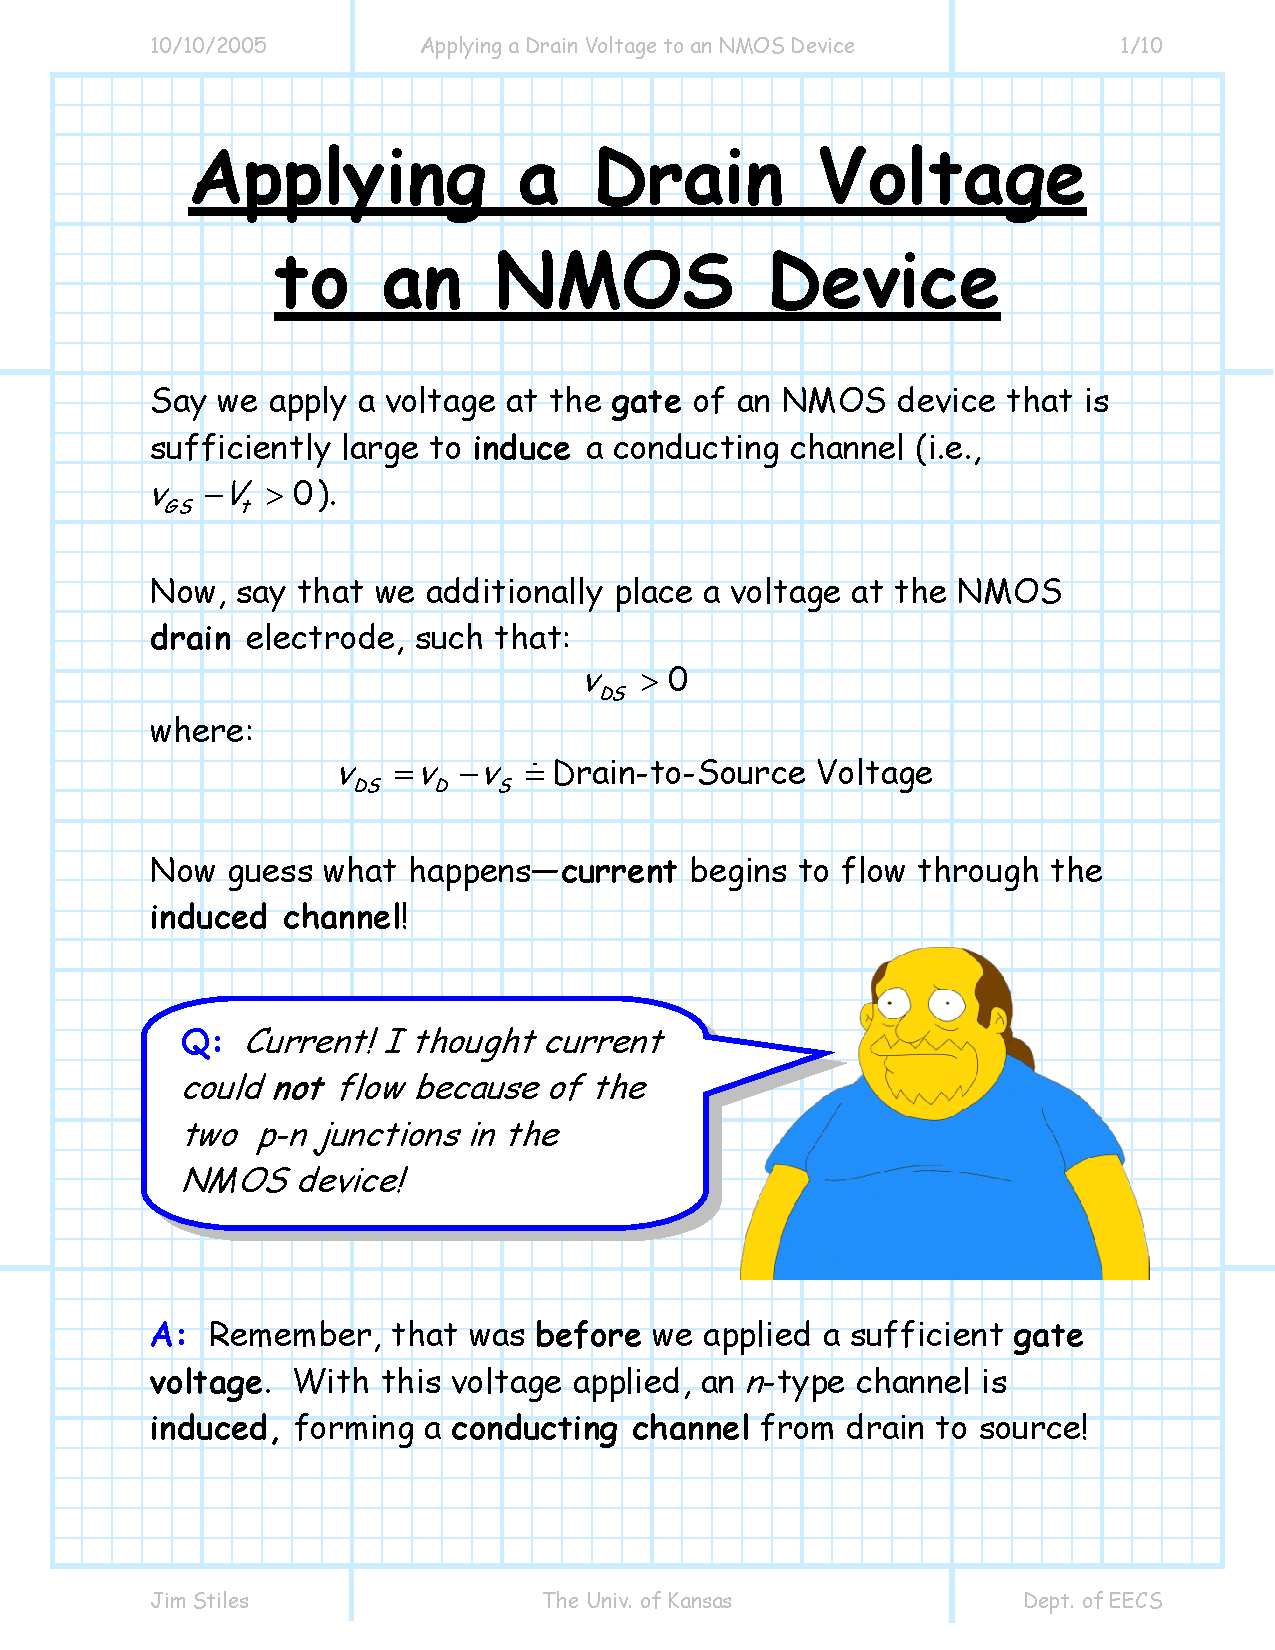
\includepdf[scale=0.9, clip, trim=10mm 10mm 10mm 10mm, pages={1-10}]{chapters/Applying_drain_voltage_nmos.pdf}


\section{Large and Small Signal Equivalent Models}
Large signal equivalent model of an $n$-channel MOSFET operating in the saturation region
\begin{figure}[H]
    \centering
    % \begin{circuitikz}[american voltages]
    %     \draw
    %       (0,0) to [short, o-] (6,0)
    %       to [V, l_=$\mathrm{j}{\omega}_m \underline{\psi}^s_R$] (6,2) 
    %       to [R, l_=$R_R$] (6,4) 
    %       to [short, i_=$\underline{i}^s_R$] (5,4) 
    %       (0,0) to [open, v^>=$\underline{u}^s_s$] (0,4) 
    %       to [short, *- ,i=$\underline{i}^s_s$] (1,4) 
    %       to [R, l=$R_s$] (3,4)
    %       to [L, l=$L_{\sigma}$] (5,4) 
    %       to [short, i_=$\underline{i}^s_M$] (5,3) 
    %       to [L, l_=$L_M$] (5,0); 
    % \end{circuitikz}
    \begin{circuitikz}[american voltages]
        \draw 
            (0,0) coordinate(a) to [short, o-o] ++(10,0) coordinate(b) 
            to (a) 
            to [open, -o] ++(0,2) coordinate(c)
            to [short,-o, i=$i_G$] ++(1,0)
            to [open, v=$v_{GS}$] ++(0,-2)
            to (b)
            to [open, v<=$v_{DS}$] ++(0,2) coordinate(d)
            to [short, i=$i_D$] ++(-1,0)
            to [short] ++(-6,0)
            to [cI, -*, l=$\frac{1}{2} k'_n \frac{W}{L}(v_{GS} - V_{tn})^2$] ++(0,-2)
            to ++(-1,0)
            to [short, *-o, l=S] ++(0,-0.5)
            to [open, -*] ++(6,0.5)
            to [R, -*, l_=$r_o$] ++(0,2)
            ;
    \end{circuitikz}
    \caption{Large signal model operating in saturation drawn with outputresistance $r_o$}
\end{figure}

Future chapters will talk about the BJT (bipolar junction transistor). 
\begin{pline}
    \item MOSFETs can be made smaller than BJTs
    \item MOSFET manufacturing process is relatively simpler and requires comparatively little powers
    \item MOSFETs generate less heat
    \item BJT better for current amplification circuits
    \item BJT low on-state voltage drop and low conduction loss
    \item BJT preferred in high power applications due to higher power handling; MOSFET preferred for low power applications
\end{pline}
\section{Practice Problems}
\begin{enumerate}
    \item Find the region of operation for the following transistors. You may use $V_{tn} = 0.9$V and $\mid V_{tp} = 1$V. The operation condition of NMOS is also shown. PMOS is conducted by holes which is opposite to NMOS so the voltage polarity is different.
    \begin{figure}[H]
        \centering
        \includegraphics[scale=0.8]{figs/ch05/pp_transistor1.png}
    \end{figure}
    \begin{center}
        \begin{tabular}{|c|c|c|}
            \hline
            Region of operation & Condsitions & \ids \\
            \hline
            Cut-off & \vgs < $V_T$ & \ids $\sim$ 0A \\
            \hline
            Linear/Triode & $V_{GS}$ > $V_T$, $V_{DS} < V_{GS} - V_T$ & \ids = {\large $\frac{W}{L} \mu_n C_{ox} (V_{GS} - V_T - \frac{V_{DS}}{2}) V_{DS}$} \\ [10pt]
            \hline
            Saturation: & $V_{GS}$ > $V_T$, $V_{DS} > V_{GS} - V_T$ & {\large \ids = $\frac{W}{L} \frac{\mu_n C_{ox}}{2} (V_{GS} - V_T)^2 (1+ \lambda V_{DS})$} \\
            \hline
        \end{tabular}
    \end{center}
    \textcolor{blue}{
    \begin{enumerate}
        \item We identify this transistor as a NMOS transistor due to the direction of the arrow. In a NMOS transistor, current flows from drain to source due to electrons being the charge carriers in the NMOS transistor. \vgs = $v_G - v_S$ = 7V and \vds = $v_D - v_S = -4 -(-8) - 4$V. This transistor is in the linear/triode region. 
        \item \vgs = 3V and \vds = 5V. This transistor is in the saturation region.
        \item This is a PMOS transistor. In a PMOS transistor, current flows from source to drain. $|v_{GS}|= 2$V and $|v_{DS}|= 0.75$V. This is in the linear/triode region.
        \item $|v_{GS}| = 4.5$V and $|v_{DS}| = |3.25 - 5| = 1.75$V. This is in the linear/triode region.
        \item $v_{GS} = 2$V and $v_{DS} = 3.25-0 = 3.25$V. This is in the saturation region.
        \item $|v_{GS}| = |4.5-5| = 0.5$V. This is in the cutoff region.
    \end{enumerate}
    }

    \item An ideal $N$-channel MOSFET has the following parameters: $W = 100$ \mun, $L = 1$ \mun, $t_{ox} = 15$ nm, the oxide relative permittivity is 4, the silicon relative permittivity is 12, $N_A = 10^{15}$\conc, $n_i = 10^{10}$\conc, $V_{FB} = -0.2$ V, $\mu_n = 300$\mobility at 300K. $\lambda = 0$.
    \begin{enumerate}
        \item Find the threshold voltage.
        \begin{Ans}
            Threshold voltage is given by the following formula:
            \begin{align*}
                \phi_B &= \frac{kT}{q} \ln\frac{N_A}{n_i} = 0.026 V \ln(\frac{10^{15} \mathrm{ cm}^{-3}}{10^{10} \mathrm{ cm}^{-3}}) = 0.2993 \dots V \\
                C_{ox} &= \frac{\epsilon_{ox}}{t_{ox}} = \frac{4(8.854 \times 10^{-14} \mathrm{F/cm})}{15 \mathrm{nm}} = 3.54 \times 10^{-7} \mathrm{F/cm}^2 \\
                V_t &= V_{FB} + 2\phi_B + \frac{\sqrt{2q\epsilon_s N_A 2 \phi_B}}{C_{ox}} \\
                &= -0.2 + 2(0.299) + \frac{2(12)(8.854 \times 10^{14} \mathrm{F/cm})(1.602 \times 10^{-19} C)(10^{15} \mathrm{cm}^{-3})(2)(0.2993 V)}{3.54 \times 10^{-7} \mathrm{F/cm}^2} \\
                &= 0.44 \mathrm{V}
            \end{align*}
        \end{Ans}

        \item What is the minumum \vds value for the MOSFET to be at saturation region at \vgs = 2V. 
        \begin{Ans}
            For the MOSFET to remain in saturation, \vds = \vgs - $V_tn$, so 
            \[V_{DS} - V_{DS} - V_{tn} = 2 - 0.44 = 1.56 \mathrm{V}\]
        \end{Ans}

        \item Find the channel resistance at \vgs = 2V and \vds = 0.01 V.
        \begin{Ans}
            Channel resistance is given by calculating what \ids is given that we know \vds is. 
            \begin{align*}
                R_{ch} &= \frac{V_{DS}}{I_{DS}} = \frac{0.01 V}{\frac{W}{L} \mu_n C_{ox} (V_{GS} - V_T) V_{DS}} \\
                &= \frac{1}{300 \times 100 \times 3.54 \times 10^{-7} \times 1.56} \\
                &= 60.36 \Omega
            \end{align*}
        \end{Ans}

        \item Find $I_D$ at \vgs = 2V and \vds = 1V.
        \begin{Ans}
            At these values, the transistor is in the linear/triode region, so 
            \begin{align*}
                I_D &= \frac{\mu_n W}{L} C_{ox} ((v_{GS} - V_{tn}) v_{DS} - \frac{v_{DS}^2}{2}) \\ 
                &= 300 \times 100 \times 3.54 \times 10^{-7}(2 - 0.44) (1 - \frac{1^2}{2}) \\
                &= 0.011 A
            \end{align*}
        \end{Ans}        

        \item Find $I_D$ at \vgs = 2V and \vds = 2V.
        \begin{Ans}
            At these values, the transistor is in the saturation region.
            \begin{align*}
                I_D &= \frac{\mu_n W}{2 L} C_{ox} (v_{gs} - v_t)^2 \\
                &= \frac{300}{2} \times 100 \times 3.54 \times 10^{-7} \times (2-0.44)^2 \\
                &= 0.013 A
            \end{align*}
        \end{Ans}
    \end{enumerate}

    \item A circuit designer intending to operate a MOSFET in saturation is considering the effect of changing the device dimensions and operating voltages on the drain current $I_D$. Specifically, by what factor does $I_D$ change in each of the following cases?
    \begin{enumerate}
        \item The channel length is doubled.
        \begin{Ans}
            The problem says that the MOSFET is in saturation. $I_D$ in saturation is 
                \[I_D = \frac{1}{2} \mu_n C_{ox} (\frac{W}{L}) (v_{GS} - V_{tn})^2\]
            From the above equation, we see that $I_D$ is inversely proportional to channel length. So, if channel length is doubled then $I_D$ will be halved.
        \end{Ans}

        \item The channel width is doubled.
        \begin{Ans}
            $I_D$ will be doubled (refer to equation for $I_D$ in saturation above).
        \end{Ans}

        \item The overdrive voltage is doubled.
        \begin{Ans}
            Overdrive voltage is equal to \vgs - $V_t$, so $I_D$ will quadruple if the overdrive voltage is doubled.
        \end{Ans}

        \item The drain to source voltage is doubled.
        \begin{Ans}
            If we doubled \vds, there will be no effect on the drain current since \vds already reaches overdrive voltage drain current saturates and remains constant.
        \end{Ans}

        \item Changes (a), (b), (c), and (d) are made simultaneously.
        \begin{Ans}
            Simultaneously doing change (a) and change (b) results in the current remaining constant. Double the overdrive voltage results in drain current quadrupling while (d) will not change drain current so the drainc current will stay 
        \end{Ans}

        \item Which of these changes might cause the MOSFET to leave the saturation region?
        \begin{Ans}
            Decreasing \vds may cause this since this may change the channel underneath.
        \end{Ans}
    \end{enumerate}
\end{enumerate}















































































































\section{Sources}
\begin{itemize}
    \item copy patse the sources from earlier chapters
\end{itemize}

% MICROELECTRONICS: AMPLIFIERS AND SIGNALS
\newpage
\chapter{Single Stage Amplifiers}
If we ignore the body terminal of the MOSFET, we have a three terminal device. Since amplifiers is a four-terminal two-port, then this means that if we use two transistors one terminal must be common with each other. This leads to the following types of single stage amplifiers:
\begin{pline}
    \item Common source (CS) amplifier
    \item Common gate (CG) amplifier 
    \item Common drain (CD) amplifier
\end{pline}
BJT equivalents, respectively, are common emitter, common base, and common collector amplifiers. 

An inductor acts as an open circuit at high frequencies due to its impedance, $j \omega L$ / $j 2 \pi L$. We see that as we increase frequency, the impedance of the inductor increases as well. To summarize. an inductor at DC is a short-circuit and at AC is an open-circuit. The opposite is true for a capacitor. For this reason, infinitely large inductors, or \textbf{chokes}, are used in place of large resistors to isolate the \textit{DC supply or reference voltages} of sensitive circuits from the rest of the noisy system. 

AC coupling capacitors are ideally infinite and blocks DC, but allows AC to flow through.

\section{Common Source Amplifier}
Has the following parameters:
\begin{pline}
    \item Can develop gain
    \item High input impedance
    \item Inverting
\end{pline}

\section{Common Gate Amplifier}
A common gate amplifier has a current gain of unity, so it acts as a \textbf{current buffer}. It must meet the following requirements:
\begin{pline}
    \item Must have a current gain of unity
    \item Should present a low input impedance
    \item Should present a high output impedance
\end{pline}

\section{Common Drain Amplifier}
The signal input comes into the gate and the signal output leaves through the source and the drain is not grounded here and is instead connected to a DC voltage. Typically used as a \textbf{voltage buffer}.

\begin{todo}
    \item Insert into appropriate section
\end{todo}

\section{Practice Problems}

\begin{enumerate}
    \item Assume that the following circuits have the same large signal operating points and that $V_{tn}$ = 1V (without body bias), $k-n = \frac{\mu C_{ox} W}{L} = 10^{-3}$ A/V\sq, $\lambda = 0$, $\gamma = 0.5$ V$^{1/2}$, and $\phi_p = $ \SI{-400}{\milli \V}. $C_{big}$ means that the AC-coupling capacitor is so large that the lower bandwidth it imposes is far below any signal we are interested in and we can treat it as a short circuit for small-signal calculations (while still keeping it an open circuit for DC biasing calculations).
    \begin{todo}
        \item do this diagram is latex when you get the chance
    \end{todo}
    
    \begin{enumerate}
        \item What amplifier configurations are circuits (a) and (b)?
        \begin{Ans}

        \end{Ans}
        
    \end{enumerate}
\end{enumerate}

\section{Sources}
\begin{itemize}
    \item EE105 Lecture 4/9/2024 by Alp Sipihigal
\end{itemize}
\end{document}